\subsection{Simulação 2}

A simulação 2 consiste em um processo de queima de um gás, no qual estão a disposição de vários sensores. Primeiramente foi descrito as entradas e saídas do sistema.

Primeiramente foi descrito as entradas e saídas do sistema por meio das tabelas \ref{tbl:3} e \ref{tbl:4}.

\begin{longtable}[]{@{}lcc@{}}
\toprule
Entradas & Nv. comportamental & Nv. tecnológico \\
\midrule
\endhead
Botão liga & \(LIG\) & LIG \\
Botão desliga & \(DES\) & DES \\
Botão de rearme & \(RES\) & RES \\
Detector de chama & \(S_C\) & S\_C \\
Sensor de fluxo de ar & \(S_A\) & S\_A \\
\bottomrule
\label{tbl:3}
\end{longtable}

\begin{longtable}[]{@{}lcc@{}}
\toprule
Saídas & Nv. comportamental & Nv. tecnológico \\
\midrule
\endhead
Ignitor & \(I\) & I \\
Motor ventilador & \(M\) & M \\
Válvula principal & \(V_{PR}\) & V\_PR \\
Válvula piloto & \(V_{PL}\) & V\_PL \\
Alarme falta-chama & \(A_{FC}\) & A\_FC \\
\bottomrule
\label{tbl:4}
\end{longtable}

Em relação aos estados das entradas e saídas, no que diz respeito aos três botões ($LIG$, $DES$ e $RES$), estes são botões normais abertos. Os sensores $S_C$ e $S_A$ identificam suas respectivas grandezas quando possuem nível lógico alto. As demais saídas ativam-se em nível lógico alto.

\begin{itemize}
    \item Etapa 0 (E0): 
    
    A etapa E0 configura-se como a etapa inicial. Ela marca inicio do processo e só transitará para a etapa E1 quando LIG tiver nível lógico alto e não haver chama acessa.
    \item Etapa 1 (E1): 
    
    Seta o motor do ventilador de ar, quando o sensor de fluxo de ar acionar passa para o E2.
    
    \item Etapa 2 (E2): 
    
    Aciona a contagem dos 20s. Após a contagem a saída auxiliar entra em nível alto passando para E3.
    
    \item Etapa 3 (E3):
    
    Nessa etapa abri-se a válvula piloto do gás e inicia a ignição por 2 segundos, quando o sensor de chama acionar passa para a etapa E4.
    
    \item Etapa 4 (E4):
    
    Nessa etapa verifica-se se há chama, se sim, abre a válvula principal de gás $V_PR$, no qual continuará ligada enquanto o botão DES não for pressionado.  
    
    \item Etapa 5 (E5):
    
    A etapa E5 é derivada da etapa E4 quando não é detectada chamas pelo sensor $S_C$, em uma situação em que o botão desliga $DES$ não é acionado.
    
    A ação executada por essa etapa é o acionamento de um alarme falta-chama $A_{FC}$ que permanecerá ativado até que um botão de rearme seja acionado e que o processo se encaminhará para o seu fim a partir da etapa E6.
    
    \item Etapa 6 (E6):
    
    A etapa E6, assim como a etapa E2 consiste em uma contagem sem nenhuma ação crítica (a menos de uma saída auxiliar para que saia do estado). O processo fica parado nessa etapa por 30 segundos para garantir que o ventilador elimine qualquer gás remanescente de queima incompleta.
    
    \item Etapa 7 (E7):

    Após a etapa E7 ser alcançada, o motor do ventilador é desligado e o processo retorna à etapa inicial quando o motor está garantidamente desligado.

\end{itemize}

\begin{figure}[H] 
\centering
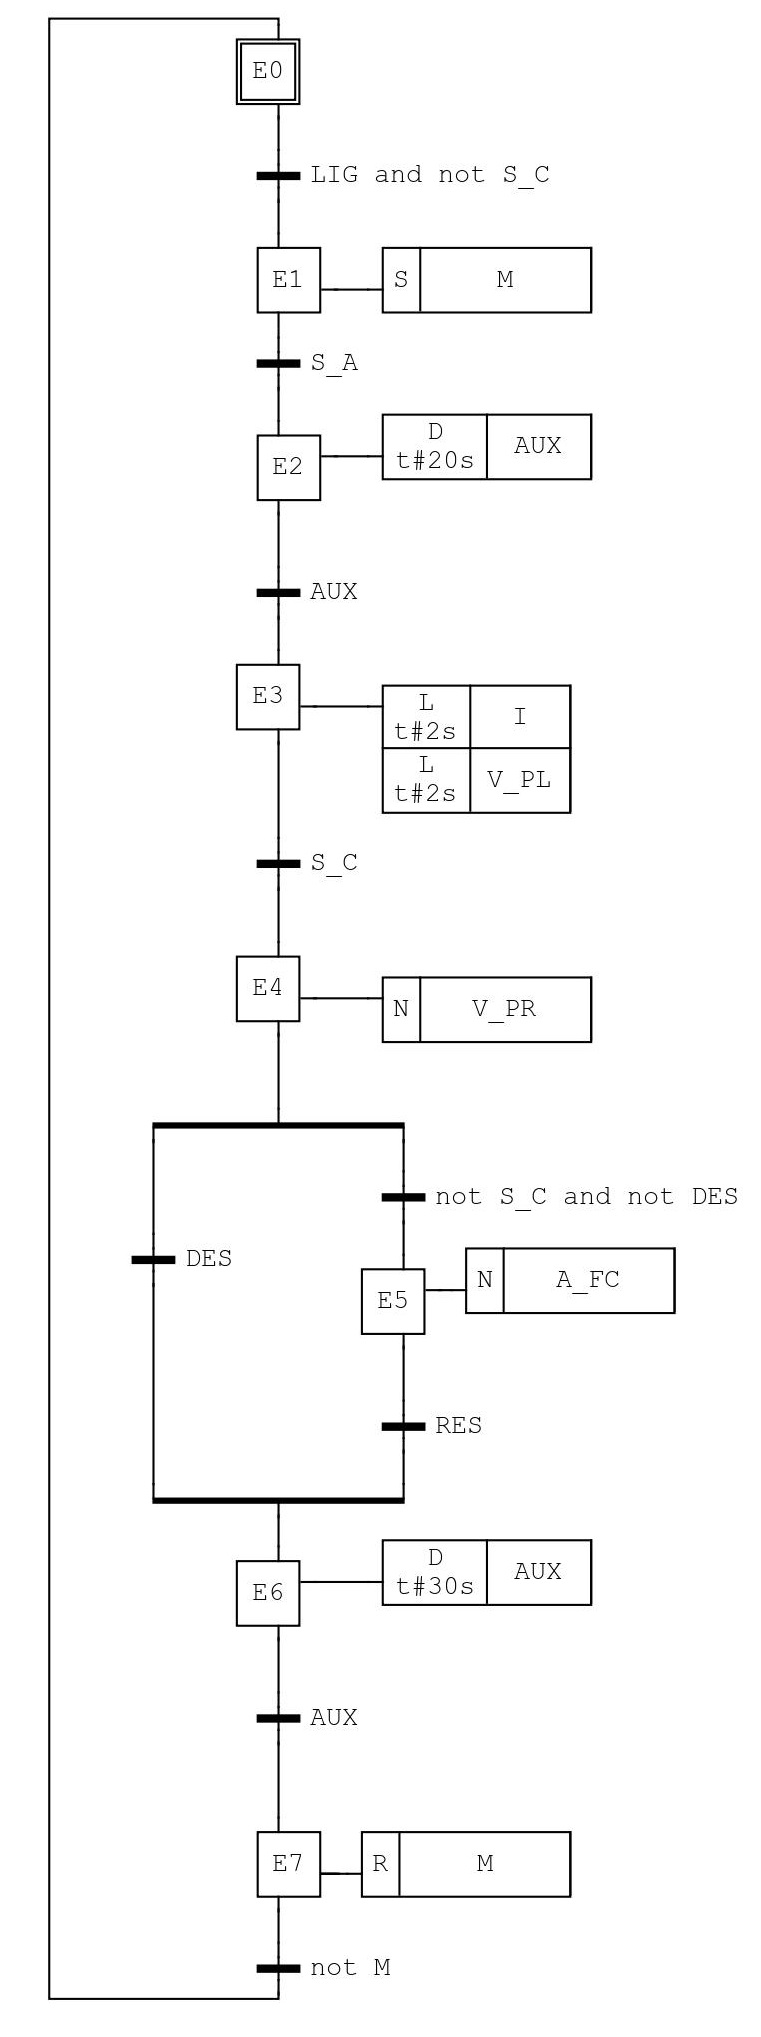
\includegraphics[width=9cm]{images/sim2.jpg}
\caption{Diagrama em SFC para a segunda simulação.}
\label{sim1]2} 
\end{figure}